\documentclass{article}


\usepackage[twoside]{fancyhdr}
\usepackage{amssymb}  % for changing bullet style
\usepackage{graphicx}
\usepackage{float}
\usepackage{hyperref}
\usepackage{url}
\usepackage{courier}
\usepackage{listings}
\usepackage{lastpage}
\usepackage[bottom]{footmisc}
\usepackage[dvipsnames]{xcolor}
\usepackage[T1]{fontenc}

\usepackage{tikz}
\usetikzlibrary{arrows.meta}

\parindent 0pt

\lstset{
	basicstyle=\ttfamily,
	breaklines=true,
	showstringspaces=false
}

\setlength{\fboxrule}{5pt}

\pagestyle{fancy}
\pagenumbering{arabic}

\fancyhead[R]{\textsc{\rightmark}}
\fancyhead[L]{}
\fancyfoot[ER,LO]{Page \thepage\ of \pageref{LastPage}}
\fancyfoot[C]{}

\renewcommand{\sectionmark}[1]{\markright{#1}{}}


\renewcommand{\headrulewidth}{2pt}
\renewcommand{\footrulewidth}{2pt}



\begin{document}
	\begin{titlepage}
		\begin{center}
		\Huge\textbf{Drawing shapes using Tikz}
		
		\vfill
		
		
\includegraphics[width=50mm]{images/intro.png}
		
		\vfill
		
		\Huge\textbf{November 5 2024}
		\end{center}
\end{titlepage}
	
	\section{Including the tikz package for drawing shapes}
	\paragraph{}
	To draw a shape in tikz, we need to use the \lstinline|tikzpicture| environment.
	
	\begin{lstlisting}[frame=tb, caption=The \lstinline|tikzpicture| environment]
\begin{tikzpicture}
	.....
\end{tikzpicture}
\end{lstlisting}
Now, in order to draw a line, we need to use the \lstinline|\draw| command as follows:

\begin{lstlisting}[frame=tb, caption=Drawing a line using tikz]
\draw (0,0)--(5,0);
\end{lstlisting}
This produces the following output:

\vspace{1cm}

\begin{tikzpicture}
\draw (0,0)--(5,0);
\end{tikzpicture}

\vspace{1cm}

The \lstinline|;| after the command indicates end of the command. Now, we can include the \lstinline|tikzpicture| within the \lstinline|center| environment as follows:

\begin{lstlisting}[frame=tb, caption=Putting \lstinline|tikzpicture| within \lstinline|center| environment]
\begin{center}
	\begin{tikzpicture}
	\draw (0,0)--(5,0);
	\end{tikzpicture}
\end{center}
\end{lstlisting}
This generates the following output:

\vspace{1cm}

\begin{center}
	\begin{tikzpicture}
	\draw (0,0)--(5,0);
	\end{tikzpicture}
\end{center}

\vspace{1cm}

The line is in the center. To change the thickness of the line, we can specify optional arguments with the \lstinline|\draw| command. Below are some listings that demonstrate how to create lines of different thickness.

\begin{lstlisting}[frame=tb, caption=Thick line]
\begin{center}
	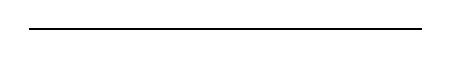
\begin{tikzpicture}
	\draw[thick] (0,0)--(5,0);
	\end{tikzpicture}
\end{center}
\end{lstlisting}
The output produced by this listing is as follows:

\begin{center}
	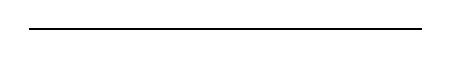
\begin{tikzpicture}
	\draw[thick] (0,0)--(5,0);
	\end{tikzpicture}
\end{center}
We can draw lines of even more thicker than this one:
\begin{lstlisting}[frame=tb, caption=A thicker line]
\begin{center}
	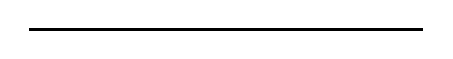
\begin{tikzpicture}
	\draw[very thick] (0,0)--(5,0);
	\end{tikzpicture}
\end{center}
\end{lstlisting}
Produces this output:


\begin{center}
	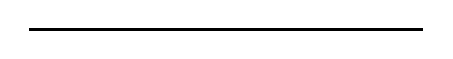
\begin{tikzpicture}
	\draw[very thick] (0,0)--(5,0);
	\end{tikzpicture}
\end{center}
If we want to specify our own value for thickness, then we can use the \lstinline|line width| option with the \lstinline|\draw| command like so:

\begin{lstlisting}[frame=tb, caption=Line of custom thickness]
\begin{center}
	
\begin{tikzpicture}
	\draw[line width=5mm] (0,0)--(5,0);
	\end{tikzpicture}
\end{center}
\end{lstlisting}
This will produce the following output:


\begin{center}
	
\begin{tikzpicture}
	\draw[line width=5mm] (0,0)--(5,0);
	\end{tikzpicture}
\end{center}
Notice that the ends of the line are sharp, we can smoothen them by using the \lstinline|cap| option like so:

\begin{lstlisting}[frame=tb, caption=Rounding the end of the line]
\begin{center}
	
\begin{tikzpicture}
	\draw[line width=5mm, cap=round] (0,0)--(5,0);
	\end{tikzpicture}
\end{center}
\end{lstlisting}
The following output is produced:


\begin{center}
	
\begin{tikzpicture}
	\draw[line width=5mm, cap=round] (0,0)--(5,0);
	\end{tikzpicture}
\end{center}
We can also change the color of the line and we don't have to use any option variables, we just need to provide the color name as an argument to \lstinline|\draw| command like so:

\begin{lstlisting}[frame=tb, caption=Changing the color of the line]
\begin{center}
	
\begin{tikzpicture}
	\draw[line width=5mm, cap=round, red] (0,0)--(5,0);
	\end{tikzpicture}
\end{center}
\end{lstlisting}
This produces the following output:

\begin{center}
	
\begin{tikzpicture}
	\draw[line width=5mm, cap=round, red] (0,0)--(5,0);
	\end{tikzpicture}
\end{center}
We can also do a color combination (with the `!') with any color. We can also create an arrow as follows:

\begin{lstlisting}[frame=tb, caption=An arrow]
\begin{center}
	
\begin{tikzpicture}
	\draw[line width=5mm, cap=round, red, ->] (0,0)--(5,0);
	\end{tikzpicture}
\end{center}
\end{lstlisting}
The \lstinline|->| means that we are drawing an arrow which looks like this:

\vspace{0.5cm}

\begin{center}
	
\begin{tikzpicture}
	\draw[line width=5mm, cap=round, red!50!brown, ->] (0,0)--(5,0);
	\end{tikzpicture}
\end{center}

\vspace{0.5cm}

There are a variety of arrows that we can draw with \lstinline|tikz|.\cite{pgfMan}

Here is the code to display another arrow:

\begin{lstlisting}[frame=tb, caption=Stealth]
\begin{center}
	
\begin{tikzpicture}
	\draw[line width=5mm, cap=round, red!50!brown, >-Stealth] (0,0)--(5,0);
	\end{tikzpicture}
\end{center}
\end{lstlisting}
This produces the following output:

\begin{center}
	
\begin{tikzpicture}
	\draw[line width=5mm, cap=round, red!50!brown, -Stealth] (0,0)--(5,0);
	\end{tikzpicture}
\end{center}
Don't forget to include the \lstinline|arrows.meta| library while drawing different variants of arrows!

\pagebreak

\bibliographystyle{plain}
\bibliography{ref}

\end{document}